\chapter{Grundlagen}
\label{grundlagen}

\section{AAL-Dienstplattform WieDAS}

\subsection{Ambient Assisted Living}

Ambient Assisted Living oder kurz AAL bezweckt eine Verschmelzung von neuen Technologien und
dem sozialen Umfeld.

Die Anzahl der Älteren und alleinstehenden Menschen in der deutschen Bevölkerung steigt stärker
als die Anzahl der jüngeren und geselligen Menschen \cite{aaldeu}.
Dieser so genannte ``Demografische Wandel'' hat als Auswirkung, dass der stärker steigende Bevölkerungsteil
mehr Pflege und Unterstützung benötigt.
Da es heutzutage immer mehr Geräte gibt, welche Menschen in jeder Lebenslage unterstützen (Fahrstühle, elektrische
Jalousien, Heizungssteuerungen, usw.) versucht AAL diesem Wandel entgegenzuwirken, indem es diese und andere neuen
Technologien im Haushalt und dem sozialen Umfeld bereitstellt.

AAL zielt dabei auf die Unterstützung im Alltag durch z.B. technische Hilfsgeräte, als auch
z.B. Diagnose und Therapie ohne das Aufsuchen eines Arztes (Telemedizin).
Daran merkt man, dass das initiale Ziel die Verbesserung der Lebensqualität von älteren
Menschen ist.
In der AAL-Umgebung finden vor Mikro- bzw. eingebettete Systeme Verwendung, da sie in der Regel
leicht in der Umgebung untergebracht werden und wenig Leistung bei gleichzeitig hoher Lebensdauer
benötigen.
Immer häufiger werden für Bedienungsgeräte auch Touchscreens verwendet, was jedoch die Lebensdauer
der Komponente stark verringert und somit nur Verwendung bei Steuerungen findet, welche nicht darauf
ausgelegt sind ständig benutzt zu werden.
Da nicht nur Benutzer, die technologiescheu sind unterstützt werden sollen, müssen AAL-Produkte
stets intuitiv und einfach in der Bedienung und Wartung sein \cite{aaldeu}, was eine Herausforderung für
die Entwickler bergt.

Die Nutzung von AAL im eigenen Wohnraum hat für Senioren und Seniorinnen zur Folge, dass sie
länger selbstständig dort verweilen können, was auch eine Entlastung des Pflegepersonals und
Pflegeaufwendungen nach sich zieht und somit auch soziale Aspekte mit sich bringt.
Das großflächige Folgeziel des AAL ist es, die Lebensqualität der Person in seinem sozialen Umfeld zu heben,
wobei der Ausgangspunkt die eigene Wohnung bildet \cite{aaldeu}.

Nicht nur ältere und alleinstehende Menschen sollen von AAL profitieren.
Durch ständige Forschung in diesem Bereich entstehen neue Konzepte und Produkte, welche wiederum
für jede Generation wertvoll sind \cite{mtidw}.
Es werden z.B. auch Kommunikationsmittel in eine AAL-Umgebung integriert (z.B. Smartphones), was
auch Menschen die gemeinschaftlich leben zu Gute kommt.
Weiterhin fördert Deutschland mit dem Bundesministerium für Bildung und Forschung AAL-Projekte,
wodurch Forschungen, Produkte und Dienstleistungen von Forschungsinstituten, Hochschulen und Firmen
stets auf Kooperation stößt und Abnehmer findet \cite{bmbf_aal}.

Eine weitere Auswirkung der Nutzung von AAL ist die Erhöhung der Sicherheit.
Beispielsweise kann einer Person, die sich vor einem Bildschirm befindet (z.B. PC oder TV),
eine derzeitige Kameraaufzeichnung eingespielt werden, sobald jemand das Grundstück betritt \cite{crestron}.

Durch den andauernden Trend des demografischen Wandels und der Weiterentwicklung von eingebetteten
Systemen bietet AAL ein großes Geschäftsfeld \cite{fhf_aal}.
Da AAL viele Möglichkeiten bietet Dienstleistungen und Produkte anzubieten und es keine technischen Standards
und Schnittstellenbeschreibungen für AAL-Produkte gibt, versuchen Hersteller sehr homogene Umgebungen
herzustellen \cite{aal_interop}.
Die Interoperabilitätsprobleme umfassen logische Problemfelder wie Bediensoftware und insbesondere Semantik
der Produkte, als auch Hardware und Kommunikationsprotokolle.

\subsection{Projektbeschreibung}
\label{gru_wiedas}

Das WieDAS (Wiesbaden-Düsseldorfer Ambient Assisted Living Service Plattform) ist eine AAL-Dienstplattform
für verteilte Assistenzsystem.
Die AAL-Dienstplattform, bietet der Software, die im Rahmen dieser Thesis beschrieben wird, den AAL-Kernaspekt,
durch Verwendung von Geräten zur Steuerung und Regelung im Wohnungsalltag.

Der Schwerpunkt des WieDAS-Projekts ist die Verwendung des verteilten Computersystems in der eigenen Wohnung,
welches zumeist aus Routern, Smartphones, Laptops und Arbeitsplatzrechnern besteht.
Das Projekt verfolgte die Entwicklung insbesondere in Hinblick auf Offenheit, Sicherheit, Erweiterbarkeit
und Mobilität der Nutzer \cite{wiedas}.

WieDAS unterliegt der Gemeinfreiheit (Public-Domain) und orientiert sich bei der Konzipierung an der
verbreiteten OSGi Dienstplattform.
Eine Interoperabilität zu vorhandenen Projekten ist jedoch eingeplant.

Besonders die Kontextsensivität und Adaptivität für bereits vorhandene AAL-Anwendungen sind besondere
Merkmale von WieDAS \cite{wiedas}.
Durch die Zusammenarbeit mit dem Fachbereich für Sozialwesen der Hochschule RheinMain, erhält das Projekt
Rückmeldung über die sozialen Aspekte des Themenfelds AAL und kann diese bei der Weiterentwicklung mit
einbeziehen.

Dem WieDAS-Projekt stehen mehrere Partner aus dem Bereich für verteilte Systeme, ambulante Dienste und
Wohnberatung zur Seite und wird bezüglich der Verwertbarkeit in Wiesbaden und Düsseldorf evaluiert \cite[Partner]{wiedas}.

\subsection{Plattform}
\label{gru_wiedas_plattform}

\begin{figure}[h]
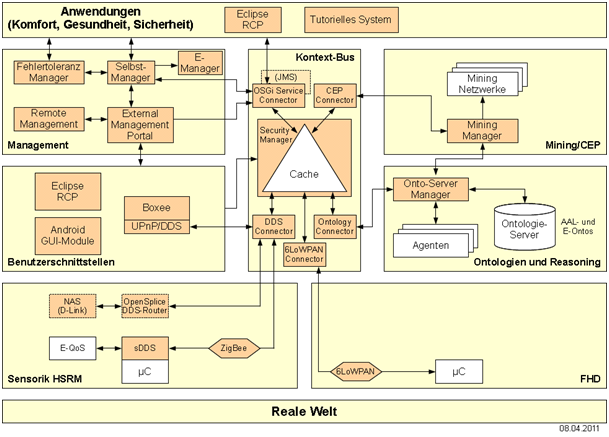
\includegraphics[scale=0.8]{images/wiedas_plattform}
\caption{WieDAS-Plattform}
\label{wiedas_plattform}
\end{figure}

Auf die WieDAS-Plattform (Abbildung \ref{wiedas_plattform}) wird von Benutzern über Anwendungen zugegriffen.
Diese Anwendungen steuern Aktoren oder liefern Mess- und Zustandsinformationen von Sensoren.
Für zusätzliche Hilfestellung beim Bedienen der Anwendungen steht in der Architektur ein
tutorielles System bereit.
Die Plattform kann über Fernwartung oder andere verbundene Management-Modulen verwaltet werden.
Weiterhin stellt die Plattform Verwaltungseinheiten für den Betrieb bereit.
Dazu gehört unter anderem das Sicherheits-Management und das anbieten virtueller fehlertolerante
Dienste, welche den implementierten Diensten überlagert sind.

Der Kern der Plattform ist der Kontext-Bus.
Er besteht aus verschiedenen Adaptermodulen (im weiteren Connectoren), welche für die WieDAS-Komponente
entwickelt werden müssen.
Die Zentraleinheit des Busses (im weiteren Cache) lagert die vorliegenden Daten und bietet sie
den angeschlossenen Modulen (Management- und Connectormodule) über eine Schnittstelle an.
Der Kontext-Bus spielt die zentrale Rolle dabei, Geräte die in der homogenen Einsatzumgebung vorkommen, zu
heterogenisieren.

Zur realen Welt liegt die Schnittstelle der Sensorik.
Hier befinden sich Sensoren, welche autarke Messwerte \cite[Plattform]{wiedas} in den WieDAS-Datenraum
befüllen.
Weitere Komponenten der Sensorik sind Aktoren, welche aus dem System heraus angesprochen werden können
und wiederum Aktionen in WieDAS selbst ausführen können.
Durch die Heterogenisierung im Kontext-Bus, soll z.B. der Sensor eines bestimmten Herstellers in der
Lage sein einen Aktor eines anderen Herstellers zu steuern oder mit Informationen zu befüllen.

Die Plattform enthält weitere Module für z.B. Mining und Reasoning, die für die Entwicklung
der Software keine Relevanz besitzen.

\subsection{AAL-Cache}
\label{gru_aalcache}

AAL-Cache ist die zentrale Softwarekomponente des Kontext-Busses des WieDAS-Projekts \ref{gru_wiedas}.

Der Kern des AAL-Cache ist die Speicherung und Erfassung von Gerätedaten aus dem Umfeld.
Damit die herstellerspezifischen Geräte und Protokolle vom AAL-Cache verarbeitet werden können, schreiben
die Softwareentwickler, die mit dem Cache arbeiten, Adaptermodule (im weiteren Connectoren).
Der Cache läuft stets dauerhaft und kann mittels der geschrieben Connectoren, welche für die
Hersteller spezifische Codestücke enthalten, Daten aus der Umgebung erfassen bzw. in diese verbreiten.
Connectoren sind Module, welche entweder zum Startzeitpunkt oder während der Laufzeit geladen werden
können.
Der AAL-Cache stellt für diese eine Schnittstelle bereit, welche wieder beim Starten der Connectoren
verwendet wird, um sich beim AAL-Cache zu registrieren.
Das Programm bedient sich dabei der Möglichkeit unter Linux dynamische Bibliotheken zu laden.

Für jeden Cache-Eintrag speichert AAL-Cache URIs in Form von Tags und binäre anwendungsspezifische Daten.
Die URIs dienen als Schlüssel und Identifikator für Cache-Einträge.
Aus Performancegründen sind die Einträge Maschinenworte.
Weiterhin speichert der Cache einige Metadaten für jedes Datum.
Darunter z.B. die Identifikation des Schreibers, Zeitstempel für die Erstellung und des letzten
Lesezugriffs des Datums, sowie der Energiebedarf zur Erhebung des Werts \cite{aalcache}.
Zum Zwecke der Lesbarkeit des Datums wird weiterhin ein Datentyp-Hint hinterlegt.

Der Cache selbst kann zur Laufzeit mittels der Management-Schnittstelle konfiguriert werden.
Initial kann der Cache mit XML-Datenstrukturen konfiguriert werden.
Darin enthalten sind z.B. Einstellungen bezüglich der Anzahl und Größte von Speicherpools und Anzahl
der bereitgestellten Cache-Einträge \cite{aalcache}.
Management-Module, welche diese Schnittstelle dann verwenden können, sind in der Lage weitere Speicherpools
anzulegen, falls die vorkonfigurierte Anzahl nicht ausreichend sein sollte.

Im aktuellen Code-Repository befinden sich bereits Connectoren für z.B. OSGi, Ontology-Homeautomation,
DDS und sDDS.

\subsection{Beschreibung der Geräte}

\section{HomeMatic}

HomeMatic ist ein Protokoll der Firma eQ-3 und wird in der Haus- und Gebäudeautomation
verwendet.
HomeMatic-Hausautomation bietet verschiedene Geräte für die Hausinstallation und wirbt damit einfach bedienbar,
zuverlässig, sicher und erweiterbar zu sein \cite{homematic_eq3}.
Das Funk-Kommunikationsprotokoll, welches für die Geräte eingesetzt wird, heißt BidCoS®.
Das Protokoll ist bidirektional und bestätigt empfangene Daten, wodurch die Sicherheit
erhöht wurde.
Es bietet jedoch weitere Sicherheitsmerkmale, z.B. die verschlüsselte Kommunikation.
Es wurde speziell für die drahtlose Ansteuerung der Geräte entwickelt \cite{homematic_eq3_faq},
wird jedoch auch für die Kommunikation über Kabelverbindungen genutzt.

\subsection{Hausautomationsgeräte}

Diese Produktserie befasst sich mit der Hausautomationstechnik und wird in mehrere
Kategorien aufgeteilt.
\begin{enumerate}
\item{Zentralen und Gateways}
\item{Sender und Controller}
\item{Sensoren}
\item{Aktoren}
\end{enumerate}

Um eine komfortable Steuerung und Verwaltung der im Haus befindlichen Geräte durchzuführen,
bietet HomeMatic Stationen an, die als Zentrale dienen.
Die Geräte in der HomeMatic-Umgebung können über Funk oder Kabel mit der Zentrale verbunden
werden.
Um die Zentrale nicht zwangsläufig am PC-Arbeitsplatz aufzustellen, bietet HomeMatic weitere
Adapter und Gateways an, um so z.B. Konfiguration mit USB-Sticks vorzunehmen.
Die Konfiguration selbst geschieht dann über das Aufrufen einer Internetanwendung, die
auf der Zentrale läuft.
Dieses Programm wird WebUI genannt \cite{homematic_webui_manual}.

Durch das Verwenden von HTTP und damit auch TCP, ist man auch in der Lage die Zentrale
über das Internet, z.B. durch die Verwendung von Smartphones zu konfigurieren.
Dazu müssen lediglich die Aufrufe aus dem Internet an die Zentrale weitergeleitet werden
(Router-Portforwarding).

HomeMatic bietet zur Ansteuerung von Aktoren moderne Funk-Fernbedienungen mit verschiedener
Anzahl von Tastern, sowie Möglichkeiten Taster in Gebäude-Elektroinstallationen Unterputz anzubringen.
Um automatisch Werte aus der Hausinstallation zu erfassen, gibt es verschiedene Sensoren für z.B.
Wetter, Rauch, Bewegung und elektrische Impulserkennung.
Als Aktoren dienen Dimmer, Unterputzeinsätze für vorhandene Installationen, einfache Ausgangsmodule und
komplexe Steuerungsmodule für z.B. Heizung oder Türgriffe.

\subsection{XML-RPC}
\label{gru_xmlrpc}

XML-RPC ist der Begriff für einen entfernten Prozeduraufruf unter der Benutzung von XML.
Es baut, wie der Name verrät, auf dem weit verbreiteten und anerkannten Interprozessprotokoll RPC
(Remote Procedure Call).
Wie der Begriff verrät, findet man RPC in verteilten Systemen, wo der Aufrufer eine gewisse
Aufgabe ausgeführt haben möchte und einen Aufruf an ein System absendet.
Der Aufrufer oder Sender wird Client und das System, welches die Aufgabe ausführt Server genannt.


Für den Programmierer ist der Aufruf selbst nicht von einem lokal ausgeführten Aufruf zu unterscheiden.
Der Programmierer sorgt lediglich für den Verbindungsaufbau zum Server.
Die Transportmechanismen sind dabei vom Programmierer versteckt und befinden sich in den jeweiligen
Implementierungen.
Für den Transport zwischen den Teilnehmern werden Nachrichten genutzt, dadurch muss die Implementierung
eine Kodierung (sogenanntes Marshalling) vornehmen.

Für dieses Marshalling bzw. den Transport selbst kann XML verwendet werden.
XML-RPC jedoch ist ein eigenständiges Protokoll, welches ein gewisses Nachrichtenformat erwartet und keine
anwendungsspezifischen Datentypen erlaubt.
Somit müssen Daten mit den vom Protokoll spezifizierten Datentypen strukturiert werden.

Während bei einer Verwendung von XML für RPC der Transportmechanismus keine Rolle spielen würde, findet
der Aufruf eines XML-RPC über HTTP statt.
Dadurch müssen die Clients und Server das HTTP Protokoll implementieren.
Ein Vorteil, welcher auch gleichzeitig ein Nachteil sein kann, ist die Einsehbarkeit der Kommunikation
von beteiligten Systemen.
Um diesem Sicherheitsmangel entgegen zu wirken, wäre eine Kommunikation über HTTPS denkbar.
